\documentclass{beamer}\usepackage[]{graphicx}\usepackage[]{xcolor}
% maxwidth is the original width if it is less than linewidth
% otherwise use linewidth (to make sure the graphics do not exceed the margin)
\makeatletter
\def\maxwidth{ %
  \ifdim\Gin@nat@width>\linewidth
    \linewidth
  \else
    \Gin@nat@width
  \fi
}
\makeatother

\definecolor{fgcolor}{rgb}{0.345, 0.345, 0.345}
\newcommand{\hlnum}[1]{\textcolor[rgb]{0.686,0.059,0.569}{#1}}%
\newcommand{\hlstr}[1]{\textcolor[rgb]{0.192,0.494,0.8}{#1}}%
\newcommand{\hlcom}[1]{\textcolor[rgb]{0.678,0.584,0.686}{\textit{#1}}}%
\newcommand{\hlopt}[1]{\textcolor[rgb]{0,0,0}{#1}}%
\newcommand{\hlstd}[1]{\textcolor[rgb]{0.345,0.345,0.345}{#1}}%
\newcommand{\hlkwa}[1]{\textcolor[rgb]{0.161,0.373,0.58}{\textbf{#1}}}%
\newcommand{\hlkwb}[1]{\textcolor[rgb]{0.69,0.353,0.396}{#1}}%
\newcommand{\hlkwc}[1]{\textcolor[rgb]{0.333,0.667,0.333}{#1}}%
\newcommand{\hlkwd}[1]{\textcolor[rgb]{0.737,0.353,0.396}{\textbf{#1}}}%
\let\hlipl\hlkwb

\usepackage{framed}
\makeatletter
\newenvironment{kframe}{%
 \def\at@end@of@kframe{}%
 \ifinner\ifhmode%
  \def\at@end@of@kframe{\end{minipage}}%
  \begin{minipage}{\columnwidth}%
 \fi\fi%
 \def\FrameCommand##1{\hskip\@totalleftmargin \hskip-\fboxsep
 \colorbox{shadecolor}{##1}\hskip-\fboxsep
     % There is no \\@totalrightmargin, so:
     \hskip-\linewidth \hskip-\@totalleftmargin \hskip\columnwidth}%
 \MakeFramed {\advance\hsize-\width
   \@totalleftmargin\z@ \linewidth\hsize
   \@setminipage}}%
 {\par\unskip\endMakeFramed%
 \at@end@of@kframe}
\makeatother

\definecolor{shadecolor}{rgb}{.97, .97, .97}
\definecolor{messagecolor}{rgb}{0, 0, 0}
\definecolor{warningcolor}{rgb}{1, 0, 1}
\definecolor{errorcolor}{rgb}{1, 0, 0}
\newenvironment{knitrout}{}{} % an empty environment to be redefined in TeX

\usepackage{alltt}
\usepackage{graphicx}
% \usepackage{comment}

\usepackage{graphicx}
\usepackage{verbatim}
\usepackage{etoolbox}
\usepackage{everysel}
% \usepackage{enumitem}

%% This package allows text highlighting
\usepackage{soul}

%% This sets the theme of the presentation which controls
%% the formatting of the slides
\usetheme{Boadilla}

%% Turn off the navigation symbols
\setbeamertemplate{navigation symbols}{} 

%% Change the default itemize [ball]s to [circle]s
\setbeamertemplate{itemize items}[circle]

%% Change the default enumerate [ball]s to plain text
\setbeamertemplate{enumerate items}[default]

%% Load the enumitem package and ensure it works nicely with beamer
% \setitemize{label=\usebeamerfont*{itemize item}
%   \usebeamercolor[fg]{itemize item}
%   \usebeamertemplate{itemize item}}
% \setenumerate{label=\usebeamerfont*{enumerate item}
%   \usebeamercolor[fg]{enumerate item}
%   \usebeamertemplate{enumerate item}}

%% Set the author block so STATS 201/8 appears on every
\author{STATS 201/8}

%% Clear the date block
\date{}


\setbeamercolor{title}{bg=blue!40}
\setbeamerfont{title}{size=\LARGE,series=\bfseries}

%%Sectioning commands
\setbeamercolor{section title}{bg=blue!20}
\setbeamerfont{section title}{size=\large}

\setbeamertemplate{section page}{%
    \begingroup
        \begin{beamercolorbox}[sep=10pt,center,rounded=true,shadow=true]{section title}
        \usebeamerfont{section title}Section~\thechapter.\thesection \newline \insertsection\par
        \end{beamercolorbox}
		\vfill
    \endgroup
}

\newcommand{\BeginSection}[1]{\section{#1} \frame{\sectionpage}}
%\AtBeginSection[]{%
%    \begin{frame}
%        \sectionpage
%    \end{frame}
%}


%% This makes all equations blue
\AtBeginEnvironment{equation*}{\color{blue}}
\AtBeginEnvironment{align*}{\color{blue}}
\everymath{\color{blue}}

%% This puts a 0 point space between paragraphs, means we don't need to use vspace, or list environments if 
%% we don't want to
\setlength{\parskip}{0pt}


%% Russell: removes spaces after R input/output?
\setlength{\topsep}{0.5mm}

%% David: In addition to Russel's command to remove spaces after R input/output, these commands remove the space between R input/output.
%% Stackoverflow link: https://stackoverflow.com/questions/35734525/reduce-space-between-code-chunks-and-code-output-in-rmarkdown-beamer-presentatio
%% \setlength{\OuterFrameSep}{-2pt}
\makeatletter
\preto{\@verbatim}{\topsep=-1pt \partopsep=-1pt }
\makeatother

%% Some useful colors
\definecolor{darkgreen}{rgb}{0.176,0.486,0.031}
\definecolor{redbrown}{HTML}{950605}
\definecolor{darkred}{HTML}{d80605}


%% nice little macro for changing the font of R code
\newcommand{\rcode}[1]{\protect{\color{darkgreen}\texttt{#1}}}

%% macro for bold blue italics
\newcommand{\blueBoldEmph}[1]{{\color{blue}\textbf{\emph{#1}}}}

% ~iid macro
\newcommand{\iid }{\stackrel{iid}{\sim}}

%% Macro for t-test amd P-value
\newcommand{\ttest}{\emph{t}-test}
\newcommand{\pval}{\emph{P}-value}

%% Statistics operators 
\DeclareMathOperator{\Bias}{Bias}
\DeclareMathOperator{\Cov}{Cov}
\DeclareMathOperator*{\Cor}{Cor}
\DeclareMathOperator{\E}{E}
\DeclareMathOperator{\MSE}{MSE}
\DeclareMathOperator{\Odds}{Odds}
\DeclareMathOperator{\OR}{OR}
\DeclareMathOperator{\PMSE}{PMSE}
\DeclareMathOperator{\sd}{sd}
\DeclareMathOperator{\se}{se}
\DeclareMathOperator*{\Var}{Var}
\DeclareMathOperator{\logit}{logit}

%% Should see if can make this a mathop
\newcommand{\comb}[2]{\mbox{$\big(_{#2}^{#1}\big)$}}



\IfFileExists{upquote.sty}{\usepackage{upquote}}{}
\begin{document}
\newcommand{\thechapter}{16}



%% Sets the document title 
\title{Chapter \thechapter: \\ Analysis of contingency tables}
\institute{University of Auckland}




\begin{frame}
\titlepage
\end{frame}


\begin{frame}[t]
\frametitle{Learning Outcomes}
In this chapter you will learn about:
\begin{center}
\vspace{16pt}
\begin{minipage}{0.95\textwidth}
  \begin{itemize}
  \item Contingency tables from grouping categorical data
  \item Modelling contingency tables using \rcode{family=binomial}
  \item Modelling contingency tables using \rcode{family=poisson}
  \item The equivalence of the binomial and Poisson models
  \item A new interpretation of odds
  \item Odds ratios (optional section)  
  \item Chi-square test of association (optional section)
  \end{itemize}
\end{minipage}
\end{center}
\end{frame}



%%%%%%%%%%%%%%%%%%%%%%%%%%%%%%%%%%%%%%%%%%%%%%%%%%%%%%%%%%%%%%%%%%%%%%%%%%%%%%%%%%%%%%%%%%%
\BeginSection{Introduction} %%%%%%%%%%%%%%%%%%%%%%%%%%%%%%%%%%%%%%%%%%%%%%%%%%%%%%%%%%%%%%%%%%%%%%%%%%%%%%%%%%%%%%%%%%%


\begin{frame}
\frametitle{Categorical data}
Count data often arise from the observation of categorical data.
\bigskip

Data are said to be ``categorical'' if the measurements made on each subject are ALL factor variables.
\bigskip

The levels of the factor variables are the ``categories'', that is, they are the distinct values that the factor variable can take.
\bigskip

The counts are then the number of times (i.e., frequencies) each combination of factor levels occurs.
\bigskip

The counts can be arranged in the form of a contingency table.
\end{frame}




\begin{frame}
\frametitle{Categorical data example\ldots}
\framesubtitle{Vaccine study}

Suppose that two vaccine treatments (Trmt A and Trmt B) are to be compared for local tenderness around the injection site. Each subject receives one of the two vaccines, and the degree of local tenderness is classified into one of four levels.

\begin{columns}
\begin{column}{0.6\textwidth}
\begin{itemize}
\setlength{\itemsep}{0mm}
\small
\item[--] no tenderness
\item[--] mild tenderness
\item[--] moderate tenderness
\item[--] severe tenderness
\end{itemize}
\end{column}

\begin{column}{0.4\textwidth}

\includegraphics[width=0.4in]{Figures/Needle.jpg}
\end{column}
\end{columns}

\bigskip

The number of each treatment-tenderness combination can then be counted and presented in the form of a contingency table:

\medskip

\begin{tabular}{c|rrrr}
          & none & mild & moderate & severe \\ \hline
Trmt A    &  21  &  16  &   11     &   2    \\
Trmt B    &   1  &  22  &   19     &   9    \\ \hline
\end{tabular}
\end{frame}



\begin{frame}
\frametitle{Categorical data example}
\framesubtitle{Hair and eye colour study}

A genetic study wanted to determine if eye colour is associated with hair colour. 
\bigskip

A large collection of randomly chosen online  portrait photographs were examined and hair and eye colour was classified as brown or not brown (other). The resulting contingency table was

\bigskip

\medskip

\begin{tabular}{c|rrrr}
              & Eyes brown & Eyes other\\ \hline
Hair brown    &  284       & 613    \\
Hair other    &  577       & 2002    \\ \hline
\end{tabular}
\end{frame}



\begin{frame}[label=Attendance1,fragile]
% \frametitle{Categorical data: Attendance/Pass example}
\frametitle{Categorical data\ldots}
\framesubtitle{Attendance/Pass}

It is of interest to examine whether attendance  of STATS 20x lectures had an association with success (pass or fail) in the course. Recall, we have data for the class of 146 students.

\bigskip

The raw format for recording categorical data is the usual rectangular format with rows being the observations on each subject, and columns being the measured factor variables. The first 8 lines of the raw data look like this:

\begin{knitrout}\scriptsize
\definecolor{shadecolor}{rgb}{0.969, 0.969, 0.969}\color{fgcolor}\begin{kframe}
\begin{alltt}
\hlstd{> }\hlstd{AP.df} \hlkwb{=} \hlkwd{read.table}\hlstd{(}\hlstr{"Data/AttendPass.txt"}\hlstd{,}\hlkwc{header}\hlstd{=T)}
\hlstd{> }\hlkwd{head}\hlstd{(AP.df,} \hlnum{8}\hlstd{)}
\end{alltt}
\begin{verbatim}
  Subject Pass     Attend
1       1 pass     attend
2       2 pass     attend
3       3 pass     attend
4       4 pass     attend
5       5 pass     attend
6       6 fail not.attend
7       7 pass not.attend
8       8 fail     attend
\end{verbatim}
\end{kframe}
\end{knitrout}

\end{frame}


\begin{frame}[fragile]
% \frametitle{Categorical data: Attendance/Pass example}
\frametitle{Categorical data\ldots}
\framesubtitle{Attendance/Pass\ldots}
The contingency table of counts can be obtained using the \rcode{table} function.
\bigskip

\begin{knitrout}\scriptsize
\definecolor{shadecolor}{rgb}{0.969, 0.969, 0.969}\color{fgcolor}\begin{kframe}
\begin{alltt}
\hlstd{> }\hlstd{AP.tbl}\hlkwb{=}\hlkwd{with}\hlstd{(AP.df,}\hlkwd{table}\hlstd{(Attend,Pass))}
\hlstd{> }\hlstd{AP.tbl}
\end{alltt}
\begin{verbatim}
            Pass
Attend       fail pass
  attend       17   83
  not.attend   27   19
\end{verbatim}
\end{kframe}
\end{knitrout}
\end{frame}



\begin{frame}[fragile]
% \frametitle{Categorical data: Attendance/Pass example}
\frametitle{Categorical data\ldots}
\framesubtitle{Attendance/Pass -- plotting the counts}
It is easy to get some useful plots of the contingency table. Since \rcode{AP.tbl} is a table, the \rcode{plot} function produces a mosaic plot:
\begin{knitrout}\scriptsize
\definecolor{shadecolor}{rgb}{0.969, 0.969, 0.969}\color{fgcolor}\begin{kframe}
\begin{alltt}
\hlstd{> }\hlkwd{plot}\hlstd{(AP.tbl,}\hlkwc{main}\hlstd{=}\hlstr{""}\hlstd{,}\hlkwc{las}\hlstd{=}\hlnum{1}\hlstd{)}
\end{alltt}
\end{kframe}
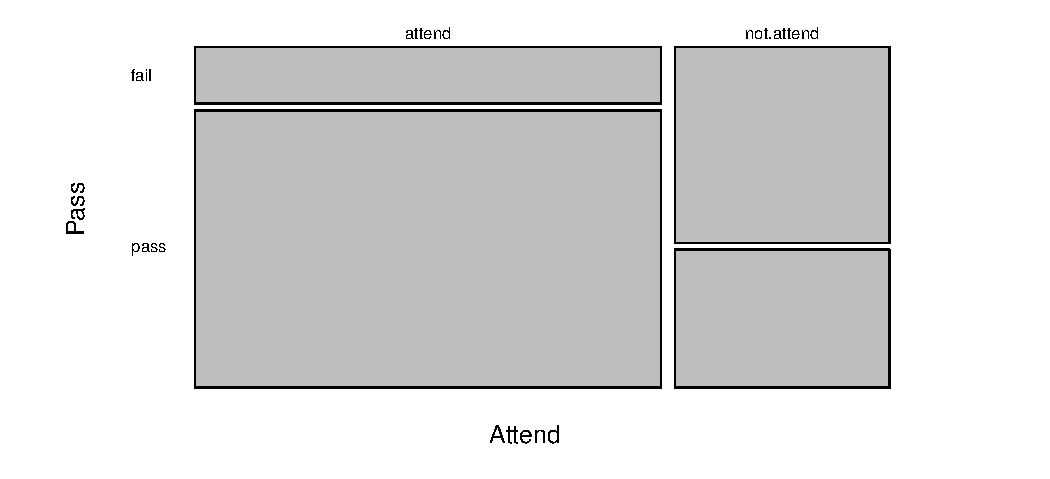
\includegraphics[width=\maxwidth]{figure/RC-H16-002b-1} 
\end{knitrout}
Note that the size of the rectangles is proportional to the count value. What does this plot tell us?
\end{frame}



\begin{frame}[fragile]
% \frametitle{Categorical data: Attendance/Pass example}
\frametitle{Categorical data\ldots}
\framesubtitle{Attendance/Pass -- plotting the counts \ldots}
The \rcode{barplot} function provides a useful bar plot:
\medskip

\begin{knitrout}\scriptsize
\definecolor{shadecolor}{rgb}{0.969, 0.969, 0.969}\color{fgcolor}\begin{kframe}
\begin{alltt}
\hlstd{> }\hlkwd{barplot}\hlstd{(}\hlkwd{t}\hlstd{(AP.tbl),}\hlkwc{legend}\hlstd{=T)}
\end{alltt}
\end{kframe}
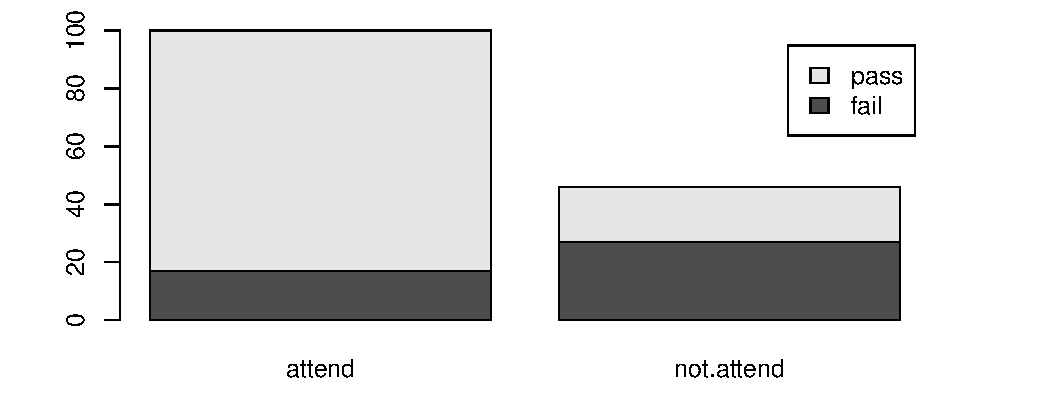
\includegraphics[width=\maxwidth]{figure/RC-H16-002c-1} 
\end{knitrout}
In the above code we used the transpose function \rcode{t} to flip the table rows and columns so that each bar would be for a level of \rcode{Attend}. If we hadn't done this the bars would have been for the levels of \rcode{Pass}, which makes interpretation harder.
\end{frame}



\begin{frame}[fragile]
% \frametitle{Categorical data: Attendance/Pass example}
\frametitle{Categorical data\ldots}
\framesubtitle{Vaccine tenderness -- plotting the counts}

\begin{knitrout}\scriptsize
\definecolor{shadecolor}{rgb}{0.969, 0.969, 0.969}\color{fgcolor}\begin{kframe}
\begin{alltt}
\hlstd{> }\hlstd{vaccines}\hlkwb{=}\hlkwd{matrix}\hlstd{(}\hlkwd{c}\hlstd{(}\hlnum{21}\hlstd{,}\hlnum{16}\hlstd{,}\hlnum{11}\hlstd{,}\hlnum{2}\hlstd{,}\hlnum{1}\hlstd{,}\hlnum{22}\hlstd{,}\hlnum{19}\hlstd{,}\hlnum{9}\hlstd{),}\hlkwc{nrow}\hlstd{=}\hlnum{2}\hlstd{,}\hlkwc{byrow}\hlstd{=T)}
\hlstd{> }\hlkwd{rownames}\hlstd{(vaccines)}\hlkwb{=}\hlkwd{c}\hlstd{(}\hlstr{"Trmt A"}\hlstd{,}\hlstr{"Trmt B"}\hlstd{)}
\hlstd{> }\hlkwd{colnames}\hlstd{(vaccines)}\hlkwb{=}\hlkwd{c}\hlstd{(}\hlstr{"none"}\hlstd{,}\hlstr{"mild"}\hlstd{,}\hlstr{"moderate"}\hlstd{,}\hlstr{"severe"}\hlstd{)}
\hlstd{> }\hlstd{vax.tbl}\hlkwb{=}\hlkwd{as.table}\hlstd{(vaccines)}
\hlstd{> }\hlstd{vax.tbl}
\end{alltt}
\begin{verbatim}
       none mild moderate severe
Trmt A   21   16       11      2
Trmt B    1   22       19      9
\end{verbatim}
\begin{alltt}
\hlstd{> }\hlkwd{plot}\hlstd{(vax.tbl,}\hlkwc{main}\hlstd{=}\hlstr{""}\hlstd{,}\hlkwc{las}\hlstd{=}\hlnum{1}\hlstd{)}
\end{alltt}
\end{kframe}
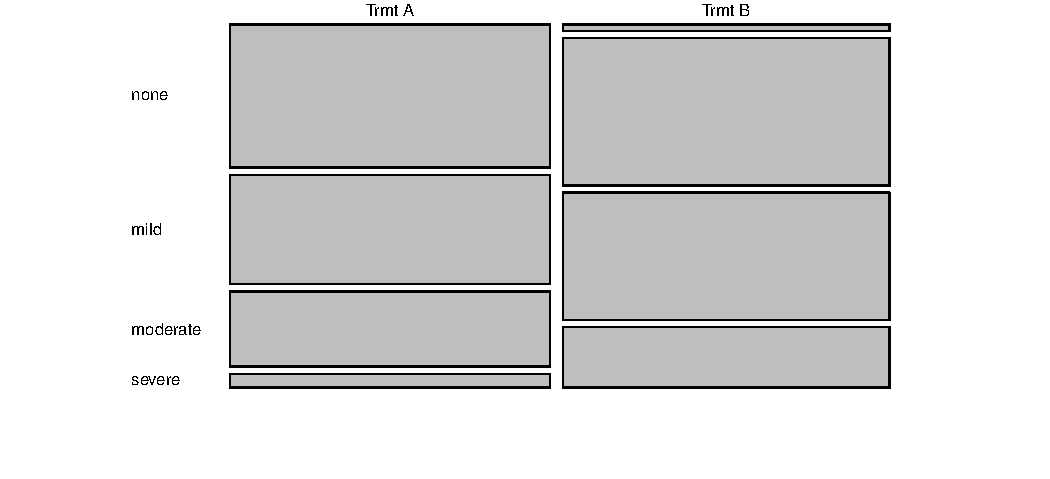
\includegraphics[width=\maxwidth]{figure/RC-H16-002d-1} 
\end{knitrout}

\end{frame}



\begin{frame}[fragile]
% \frametitle{Categorical data: Attendance/Pass example}
\frametitle{Categorical data\ldots}
\framesubtitle{Vaccine tenderness -- plotting the counts \ldots}
The \rcode{barplot} function is not very good at placing the legend!
\medskip

\begin{knitrout}\scriptsize
\definecolor{shadecolor}{rgb}{0.969, 0.969, 0.969}\color{fgcolor}\begin{kframe}
\begin{alltt}
\hlstd{> }\hlkwd{barplot}\hlstd{(}\hlkwd{t}\hlstd{(vax.tbl),}\hlkwc{ylim}\hlstd{=}\hlkwd{c}\hlstd{(}\hlnum{0}\hlstd{,}\hlnum{70}\hlstd{),}\hlkwc{legend}\hlstd{=T)}
\end{alltt}
\end{kframe}
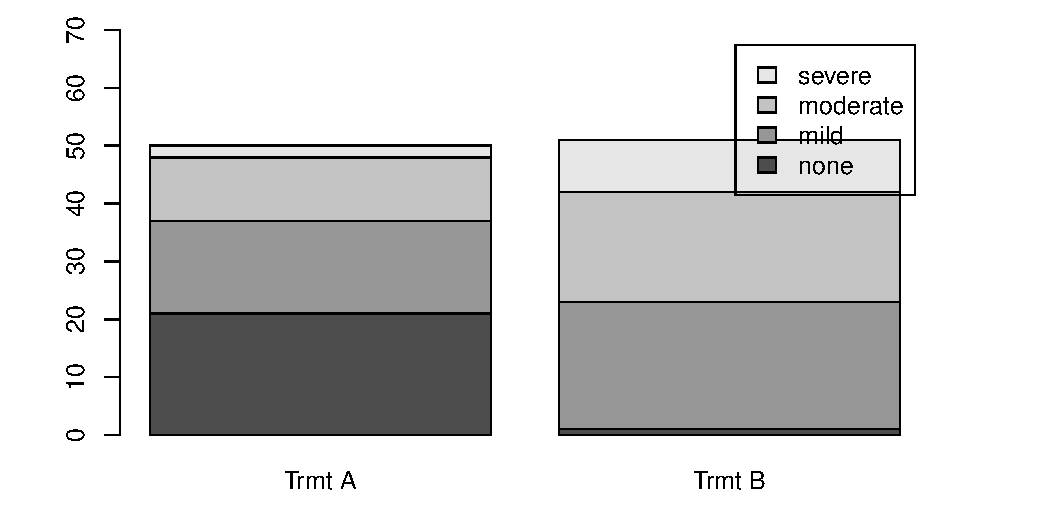
\includegraphics[width=\maxwidth]{figure/RC-H16-002e-1} 
\end{knitrout}

For the vaccine data there are an equal number of subject in both treatments, so the mosaic plot and barplot are the same (other than the bars being stacked in reverse order)
\end{frame}




\begin{frame}[fragile]
\frametitle{Remark 1}
In each of the above examples the frequencies were presented in the form a two-way (i.e., by row and by column) contingency table.
\bigskip

The contingency table was 2-by-4 for the vaccine study, and 2-by-2 in the hair/eye colour and attendance/pass example. In general, the number of rows and columns in a two-way contingency table is given by the number of levels of the corresponding factors.
\bigskip

More generally, if $s$ factor variables are recorded on each subject then the resulting table will be a $s$-way contingency table, with dimensions given by the number of levels of each of the $s$ factors.
\vfill
\end{frame}



\begin{frame}[fragile]
\frametitle{Remark 2}
With categorical data, it may or may not be possible to identify some of the factor variables as explanatory variables and some as response variables.
\bigskip

It totally depends on the particular situation:

\begin{itemize}
  \item The vaccine study was conducted to see if tenderness depends on which vaccine treatment was given, so it is clear that treatment is the explanatory variable, and the measured tenderness is the response.
  \item In the hair/eye colour example neither is clearly an explanatory or response.
  \item In the attendance/pass example it is natural to consider attendance as an explanatory variable for pass, and indeed we have already done that in this course.
\end{itemize}
\end{frame}



\begin{frame}[fragile]
\frametitle{Remark 3}
With categorical data, it may or may not be possible to say whether the counts are from a fixed number of trials (e.g., binomial data), or are more like Poisson data.
\bigskip

\begin{itemize}
  \item In the vaccine example it is most likely that there was a fixed number of treatments applied, so if we created a dichotomous response (such as, "no tenderness" or "some tenderness") then we could model it as binomial.
  \item In the hair/eye colour example there is no clear notion of a fixed number of trials for any hair or eye colour.
  \item In the attendance/pass example:
  \begin{itemize}
    \item One could say that the number of attenders and non-attenders was fixed (at 100 and 46, respectively) prior to the exam.
    \item Alternatively, one could argue that the the number of attenders and non-attenders was not fixed since it depended on the number of enrolments.
  \end{itemize}
\end{itemize}


\end{frame}



\begin{frame}[fragile]
\frametitle{Remarks}
The last two slides above note some interesting properties of categorical data. As we shall see, these considerations don't matter to our analysis -- but they may determine our interpretation.
\bigskip

The underlying research question is to establish whether or not there is an association between the factors.
\medskip

If there is an association then we would also like to be able to quantify it.

\bigskip \bigskip

NOTE: This Chapter concludes with a recap of the methodology seen in STATS 10x for testing for association in contingency tables -- the chi-squared test for association. Your lecturer will advise whether it is examinable.
\end{frame}



%%%%%%%%%%%%%%%%%%%%%%%%%%%%%%%%%%%%%%%%%%%%%%%%%%%%%%%%%%%%%%%%%%%%%%%%%%%%%%%%%%%%%%%%%%%
\BeginSection{The binomial approach to contingency table analysis} %%%%%%%%%%%%%%%%%%%%%%%%%%%%%%%%%%%%%%%%%%%%%%%%%%%%%%%%%%%%%%%%%%%%%%%%%%%%%%%%%%%%%%%%%%%


\begin{frame}[fragile]
\frametitle{Attendance/Pass}
Two STATS 20x students, Kim and Des, have been assigned to the task of determining whether there is an association between attendance and exam success in STATS 20X. 
\medskip

Kim has decided to use the binomial approach to analyse the data -- this makes sense, since we can regard attendance as an explanatory variable, and pass/fail as a Bernoulli outcome.
\medskip

We'll help Kim out by creating a dataframe in the format needed for a binomial GLM.

%Using table object in glm is tricky. Construct df from scratch.
\begin{knitrout}\scriptsize
\definecolor{shadecolor}{rgb}{0.969, 0.969, 0.969}\color{fgcolor}\begin{kframe}
\begin{alltt}
\hlstd{> }\hlstd{Freqs.df} \hlkwb{=} \hlkwd{data.frame}\hlstd{(}\hlkwc{Attend}\hlstd{=}\hlkwd{c}\hlstd{(}\hlstr{"not.attend"}\hlstd{,}\hlstr{"attend"}\hlstd{),}\hlkwc{Fail}\hlstd{=}\hlkwd{c}\hlstd{(}\hlnum{27}\hlstd{,}\hlnum{17}\hlstd{),}\hlkwc{Pass}\hlstd{=}\hlkwd{c}\hlstd{(}\hlnum{19}\hlstd{,}\hlnum{83}\hlstd{))}
\hlstd{> }\hlstd{Freqs.df} \hlkwb{=} \hlkwd{transform}\hlstd{(Freqs.df,}\hlkwc{Attend}\hlstd{=}\hlkwd{factor}\hlstd{(Attend))}
\hlstd{> }\hlstd{Freqs.df}
\end{alltt}
\begin{verbatim}
      Attend Fail Pass
1 not.attend   27   19
2     attend   17   83
\end{verbatim}
\end{kframe}
\end{knitrout}
\medskip

If an association is detected then Kim also needs to quantity the strength of the assocation with a suitable confidence interval.
\medskip

\end{frame}



\begin{frame}[fragile]
\frametitle{Attendance/Pass\ldots}
\framesubtitle{Binomial analysis}
Kim decides to change the reference level of \rcode{Attend} to \rcode{not.attend} so that any effect can be expressed as the effect of attending.
\bigskip



Fitting the binomial GLM is easy:
\begin{knitrout}\scriptsize
\definecolor{shadecolor}{rgb}{0.969, 0.969, 0.969}\color{fgcolor}\begin{kframe}
\begin{alltt}
\hlstd{> }\hlstd{AP.binom}\hlkwb{=}\hlkwd{glm}\hlstd{(}\hlkwd{cbind}\hlstd{(Pass,Fail)}\hlopt{~}\hlstd{Attend,}\hlkwc{data}\hlstd{=Freqs.df,}\hlkwc{family}\hlstd{=binomial)}
\hlstd{> }\hlkwd{summary}\hlstd{(AP.binom)}
\end{alltt}
\end{kframe}
\end{knitrout}

\begin{knitrout}\scriptsize
\definecolor{shadecolor}{rgb}{0.969, 0.969, 0.969}\color{fgcolor}\begin{kframe}
\begin{verbatim}
Call:
glm(formula = cbind(Pass, Fail) ~ Attend, family = binomial, 

Coefficients:
             Estimate Std. Error z value Pr(>|z|)    
(Intercept)   -0.3514     0.2994  -1.173    0.241    
Attendattend   1.9370     0.4007   4.834 1.34e-06 ***
---
(Dispersion parameter for binomial family taken to be 1)

    Null deviance:  2.5162e+01  on 1  degrees of freedom
Residual deviance: -4.2188e-15  on 0  degrees of freedom
\end{verbatim}
\end{kframe}
\end{knitrout}
\end{frame}



\begin{frame}[fragile]
\frametitle{Attendance/Pass\ldots}
\framesubtitle{Binomial analysis\ldots}

Note that the residual deviance is zero, on zero degrees of freedom -- this is nothing to worry about.\footnote{The data consist of two observations, and the model fits two parameters, so there are no degrees of freedom left.}
\bigskip

The effect of \rcode{Attend} is highly significant, so let's calculate a CI:

\begin{knitrout}\scriptsize
\definecolor{shadecolor}{rgb}{0.969, 0.969, 0.969}\color{fgcolor}\begin{kframe}
\begin{alltt}
\hlstd{> }\hlkwd{exp}\hlstd{(}\hlkwd{confint}\hlstd{(AP.binom))[}\hlnum{2}\hlstd{,]}
\end{alltt}


{\ttfamily\noindent\itshape\color{messagecolor}{Waiting for profiling to be done...}}\begin{verbatim}
    2.5 %    97.5 % 
 3.214049 15.552487 
\end{verbatim}
\end{kframe}
\end{knitrout}
\bigskip

So, Kim concludes that the odds of an attender passing STATS 20x are between 3.2 and 15.6 times the odds of a non-attender passing. Yikes!
\end{frame}


%%%%%%%%%%%%%%%%%%%%%%%%%%%%%%%%%%%%%%%%%%%%%%%%%%%%%%%%%%%%%%%%%%%%%%%%%%%%%%%%%%%%%%%%%%%
\BeginSection{The Poisson approach to contingency table analysis} %%%%%%%%%%%%%%%%%%%%%%%%%%%%%%%%%%%%%%%%%%%%%%%%%%%%%%%%%%%%%%%%%%%%%%%%%%%%%%%%%%%%%%%%%%%

\begin{frame}[fragile]
\frametitle{Attendance/Pass\ldots}
\framesubtitle{Poisson analysis}
The other student, Des, feels that the frequencies are best modeled as Poisson counts because the number of students was not fixed at the start of the semester, and depended on the whims of enrolment.
\medskip

Des needs the data in the following format:
\medskip

\begin{knitrout}\scriptsize
\definecolor{shadecolor}{rgb}{0.969, 0.969, 0.969}\color{fgcolor}\begin{kframe}
\begin{alltt}
\hlstd{> }\hlkwd{library}\hlstd{(dplyr)}
\hlstd{> }\hlstd{AP.df} \hlkwb{=} \hlkwd{read.table}\hlstd{(}\hlstr{"Data/AttendPass.txt"}\hlstd{,}\hlkwc{header}\hlstd{=T)}
\hlstd{> }\hlstd{AP.df} \hlkwb{=} \hlkwd{transform}\hlstd{(AP.df,} \hlkwc{Pass}\hlstd{=}\hlkwd{factor}\hlstd{(Pass),} \hlkwc{Attend}\hlstd{=}\hlkwd{factor}\hlstd{(Attend))}
\hlstd{> }\hlstd{Freqs2.df} \hlkwb{=} \hlstd{AP.df} \hlopt \hlkwd{group_by}\hlstd{(Attend,Pass)} \hlopt \hlkwd{summarize}\hlstd{(}\hlkwc{freq}\hlstd{=}\hlkwd{n}\hlstd{())} \hlopt
\hlstd{+ }                   \hlkwd{data.frame}\hlstd{()}
\hlstd{> }\hlstd{Freqs2.df}
\end{alltt}
\begin{verbatim}
      Attend Pass freq
1     attend fail   17
2     attend pass   83
3 not.attend fail   27
4 not.attend pass   19
\end{verbatim}
\end{kframe}
\end{knitrout}
\end{frame}


\begin{frame}[fragile]
\frametitle{Attendance/Pass\ldots}
\framesubtitle{Poisson analysis\ldots}
Des fits the interaction model to check for an association between attendance and passing.\footnote{That is, to see if the expected numbers in the \rcode{pass} group relative to the \rcode{fail} group depend on attendance.} He also relevels \rcode{Attend}.


\begin{knitrout}\scriptsize
\definecolor{shadecolor}{rgb}{0.969, 0.969, 0.969}\color{fgcolor}\begin{kframe}
\begin{alltt}
\hlstd{> }\hlstd{Freqs2.df}\hlopt{$}\hlstd{Attend}\hlkwb{=}\hlkwd{relevel}\hlstd{(Freqs2.df}\hlopt{$}\hlstd{Attend,} \hlkwc{ref}\hlstd{=}\hlstr{"not.attend"}\hlstd{)}
\hlstd{> }\hlstd{AP.pois}\hlkwb{=}\hlkwd{glm}\hlstd{(freq}\hlopt{~}\hlstd{Attend}\hlopt{*}\hlstd{Pass,}\hlkwc{family}\hlstd{=poisson,}\hlkwc{data}\hlstd{=Freqs2.df)}
\hlstd{> }\hlkwd{summary}\hlstd{(AP.pois)}
\end{alltt}
\end{kframe}
\end{knitrout}

\begin{knitrout}\scriptsize
\definecolor{shadecolor}{rgb}{0.969, 0.969, 0.969}\color{fgcolor}\begin{kframe}
\begin{verbatim}
Call:
glm(formula = freq ~ Attend * Pass, family = poisson, data = Freqs2.df)

Coefficients:
                      Estimate Std. Error z value Pr(>|z|)    
(Intercept)             3.2958     0.1925  17.126  < 2e-16 ***
Attendattend           -0.4626     0.3096  -1.494    0.135    
Passpass               -0.3514     0.2994  -1.173    0.241    
Attendattend:Passpass   1.9370     0.4007   4.834 1.34e-06 ***
---
(Dispersion parameter for poisson family taken to be 1)

    Null deviance:  6.9305e+01  on 3  degrees of freedom
Residual deviance: -3.9968e-15  on 0  degrees of freedom
\end{verbatim}
\end{kframe}
\end{knitrout}
\end{frame}



\begin{frame}[fragile]
\frametitle{Attendance/Pass\ldots}
\framesubtitle{Poisson analysis\ldots}
As with the binomial model,the residual deviance is zero, on zero degrees of freedom. Again, this is nothing to worry about.\footnote{The data consist of four observed counts, and the model fits four parameters, so there are no degrees of freedom left.}
\medskip

Note that the interaction effect is highly significant.
In fact, {\bf the \rcode{Attend:Pass} interaction effect from Des's Poisson analysis is exactly the same as the \rcode{Attend} effect from Kim's binomial analysis}.  
\bigskip 

The CI for $\exp(\beta_3)$ from the Poisson model is identical to Kim's CI
\medskip

\begin{knitrout}\scriptsize
\definecolor{shadecolor}{rgb}{0.969, 0.969, 0.969}\color{fgcolor}\begin{kframe}
\begin{alltt}
\hlstd{> }\hlkwd{exp}\hlstd{(}\hlkwd{confint}\hlstd{(AP.pois))[}\hlnum{4}\hlstd{,]}
\end{alltt}


{\ttfamily\noindent\itshape\color{messagecolor}{Waiting for profiling to be done...}}\begin{verbatim}
    2.5 %    97.5 % 
 3.214049 15.552487 
\end{verbatim}
\end{kframe}
\end{knitrout}
\medskip

The next section shows why these two different models produce the same estimate.

\end{frame}



%%%%%%%%%%%%%%%%%%%%%%%%%%%%%%%%%%%%%%%%%%%%%%%%%%%%%%%%%%%%%%%%%%%%%%%%%%%%%%%%%%%%%%%%%%%
\BeginSection{Equivalence of the binomial and Poisson approaches} %%%%%%%%%%%%%%%%%%%%%%%%%%%%%%%%%%%%%%%%%%%%%%%%%%%%%%%%%%%%%%%%%%%%%%%%%%%%%%%%%%%%%%%%%%%


\begin{frame}
\frametitle{Equivalence of binomial and Poisson approaches}
Consider the 2-by-2 contingency table:
\medskip

\begin{center}
{\tt \small 
\begin{tabular}{rr}
$n_{11}$ & $n_{12}$   \\
$n_{21}$ & $n_{22}$   \\ 
\end{tabular}}
\end{center}
\bigskip

We'll assume that row 1 and column 1 correspond to the reference levels for the row and column factor variables, respectively.
\medskip

Then, from Chapters 13 and 14, the Poisson interaction model\footnote{Here we assume the model \rcode{ glm(n $\sim$ RowVar * ColVar, family=poisson)} where \rcode{RowVar} and \rcode{ColVar} are the row and column factor variables, respectively.} for these data is
\medskip


\begin{itemize}
\item[] $\log \E[n_{11}] = \beta_0$ 
\item[] $\log \E[n_{21}] = \beta_0 + \beta_1$ 
\item[] $\log \E[n_{12}] = \beta_0 + \beta_2$ 
\item[] $\log \E[n_{22}] = \beta_0 + \beta_1 + \beta_2 + \beta_3$
\end{itemize}

\end{frame}



\begin{frame}
\frametitle{Equivalence of binomial and Poisson approaches\ldots}
\framesubtitle{An odds interpretation\ldots}
Equivalently,
\medskip

\begin{itemize}
\item[] $\E[n_{11}] = \exp(\beta_0)$
\item[] $\E[n_{21}] = \exp(\beta_0 + \beta_1)$
\item[] $\E[n_{12}] = \exp(\beta_0 + \beta_2) = \E[n_{11}] \times \exp(\beta_2)$
\item[] $\E[n_{22}] = \exp(\beta_0 + \beta_1 + \beta_2 + \beta_3) = \E[n_{21}] \times \exp(\beta_2 + \beta_3)$ 
\end{itemize}
\bigskip

So, we can say that for every one occurrence expected in the $[1,1]$ cell we expect $\exp(\beta_2)$  occurrences in the $[1,2]$ cell. 
\medskip

Another way of interpreting this is that within row 1, an occurrence is $\exp(\beta_2)$ times as likely to be in column 2 than column 1. 
\medskip

What we've just said is that, within row 1, the odds of being in column 2 (rather than column 1) is $\exp(\beta_2)$.\footnote{Recall this example from Chapter 15: If the odds of A are 2 (i.e., 2-to-1) then we are saying that A is twice as likely to occur as not. That is Pr(A)=2/3 and Pr(not A)=1/3.}
\end{frame}



\begin{frame}[fragile]
\frametitle{Equivalence of binomial and Poisson approaches\ldots}
\framesubtitle{An odds interpretation\ldots}
Let's compare the expected occurrences in the $[2,1]$ and $[2,2]$ cells.
\medskip

Within row 2, an occurrence is $\exp(\beta_2 + \beta_3)$ times as likely  to be in column 2 than column 1. 
\medskip

That is, within row 2, the odds of being in column 2 (rather than column 1) is $\exp(\beta_2 + \beta_3) = \exp(\beta_2) \times \exp(\beta_3)$.
\bigskip

Note that the multiplicative change in column 2 odds between row 2 and row 1 is $\exp(\beta_3)$. 

\end{frame}



\begin{frame}[fragile]
\frametitle{Attendance/Pass\ldots}
\framesubtitle{Equivalence of binomial and Poisson approaches\ldots}
Recall, our contingency table for this example is
\medskip
\begin{knitrout}\scriptsize
\definecolor{shadecolor}{rgb}{0.969, 0.969, 0.969}\color{fgcolor}\begin{kframe}
\begin{alltt}
\hlstd{> }\hlstd{Freqs.df}
\end{alltt}
\begin{verbatim}
      Attend Fail Pass
1 not.attend   27   19
2     attend   17   83
\end{verbatim}
\end{kframe}
\end{knitrout}
\medskip

and the CI for $\exp(\beta_3)$ from the Poisson model is
\medskip

\begin{knitrout}\scriptsize
\definecolor{shadecolor}{rgb}{0.969, 0.969, 0.969}\color{fgcolor}\begin{kframe}
\begin{alltt}
\hlstd{> }\hlkwd{exp}\hlstd{(}\hlkwd{confint}\hlstd{(AP.pois))[}\hlnum{4}\hlstd{,]}
\end{alltt}


{\ttfamily\noindent\itshape\color{messagecolor}{Waiting for profiling to be done...}}\begin{verbatim}
    2.5 %    97.5 % 
 3.214049 15.552487 
\end{verbatim}
\end{kframe}
\end{knitrout}
\bigskip

We now have the same interpretation from the Poisson model as from the binomial model --
the odds of an attender (row 2) passing STATS 20x (column 2) are between 3.2 and 15.6 times the odds of a non-attender passing.

\end{frame}


%%%%%%%%%%%%%%%%%%%%%%%%%%%%%%%%%%%%%%%%%%%%%%%%%%%%%%%%%%%%%%%%%%%%%%%%%%%%%%%%%%%%%%%%%%%
\BeginSection{Closing remarks} %%%%%%%%%%%%%%%%%%%%%%%%%%%%%%%%%%%%%%%%%%%%%%%%%%%%%%%%%%%%%%%%%%%%%%%%%%%%%%%%%%%%%%%%%%%


\begin{frame}[fragile]
\frametitle{Equivalence of binomial and Poisson approaches\ldots}
\framesubtitle{Closing remarks}
The binomial and Poisson models fitted above are so-called {\em saturated} models because there are as many parameters as there are observations, and hence zero degrees of freedom.
\bigskip

A saturated model has perfect fit. To see that, let's look at the fitted counts from the Poisson model fitted to \rcode{Freqs2.df}.
\medskip

\begin{knitrout}\scriptsize
\definecolor{shadecolor}{rgb}{0.969, 0.969, 0.969}\color{fgcolor}\begin{kframe}
\begin{alltt}
\hlstd{> }\hlkwd{predict}\hlstd{(AP.pois,}\hlkwc{type}\hlstd{=}\hlstr{"response"}\hlstd{)}
\end{alltt}
\begin{verbatim}
 1  2  3  4 
17 83 27 19 
\end{verbatim}
\begin{alltt}
\hlstd{> }\hlstd{Freqs2.df}
\end{alltt}
\begin{verbatim}
      Attend Pass freq
1     attend fail   17
2     attend pass   83
3 not.attend fail   27
4 not.attend pass   19
\end{verbatim}
\end{kframe}
\end{knitrout}

The fitted counts are exactly the observed counts -- a perfect fit!

\end{frame}



\begin{frame}[fragile]
\frametitle{Equivalence of binomial and Poisson approaches\ldots}
\framesubtitle{Closing remarks}
\begin{itemize}
  \item The odds interpretation that we are using for Poisson analysis of contingency tables is generally not appropriate for the other types of Poisson count data that were seen in Chapters 13 and 14.\footnote{You will lose marks if used inappropriately.} \medskip
  
  \item The odds multiplier was $\exp(\beta_1)$ from the binomial model, and equivalently $\exp(\beta_3)$ from the Poisson model. This is commonly called the  {\bf odds-ratio}. E.g., in row 2 the odds-ratio (relative to row 1) for the column 2 outcome is between 3.2 and 15.6. \medskip
  
  \item In practice, the {\bf Poisson approach is most widely used} because
  \begin{itemize}
    \item The binomial approach is limited to a binary response category.
    \item The Poisson approach can handle tables of arbitrary number of row and/or columns.
    \item The Poisson approach can handle multi-way tables.
    \item The Poisson approach can test other types of hypotheses, e.g., that all row outcomes are equally likely.
  \end{itemize}
\end{itemize}
\end{frame}



%%%%%%%%%%%%%%%%%%%%%%%%%%%%%%%%%%%%%%%%%%%%%%%%%%%%%%%%%%%%%%%%%%%%%%%%%%%%%%%%%%%%%%%%%%%
\BeginSection{Odds ratios \\ ~ \\
(This is an optional Section \\ - your lecturer will advise if it is examinable)} %%%%%%%%%%%%%%%%%%%%%%%%%%%%%%%%%%%%%%%%%%%%%%%%%%%%%%%%%%%%%%%%%%%%%%%%%%%%%%%%%%%%%%%%%%%



\begin{frame}[fragile]
\frametitle{Odds ratios}
Recall, the contingency table for the attendance/pass example is

\begin{knitrout}\scriptsize
\definecolor{shadecolor}{rgb}{0.969, 0.969, 0.969}\color{fgcolor}\begin{kframe}
\begin{alltt}
\hlstd{> }\hlstd{Freqs.df}
\end{alltt}
\begin{verbatim}
      Attend Fail Pass
1 not.attend   27   19
2     attend   17   83
\end{verbatim}
\end{kframe}
\end{knitrout}
\medskip

and the fitted Poisson model is
\begin{knitrout}\scriptsize
\definecolor{shadecolor}{rgb}{0.969, 0.969, 0.969}\color{fgcolor}\begin{kframe}
\begin{alltt}
\hlstd{> }\hlkwd{coef}\hlstd{(}\hlkwd{summary}\hlstd{(AP.pois))}
\end{alltt}
\begin{verbatim}
                        Estimate Std. Error   z value     Pr(>|z|)
(Intercept)            3.2958369  0.1924501 17.125671 9.550242e-66
Attendattend          -0.4626235  0.3096136 -1.494197 1.351243e-01
Passpass              -0.3513979  0.2994472 -1.173489 2.405999e-01
Attendattend:Passpass  1.9370252  0.4006749  4.834407 1.335434e-06
\end{verbatim}
\end{kframe}
\end{knitrout}
\medskip
Our estimated value of the odds-ratio is therefore

\begin{knitrout}\scriptsize
\definecolor{shadecolor}{rgb}{0.969, 0.969, 0.969}\color{fgcolor}\begin{kframe}
\begin{alltt}
\hlstd{> }\hlkwd{exp}\hlstd{(}\hlkwd{coef}\hlstd{(AP.pois))[}\hlnum{4}\hlstd{]}
\end{alltt}
\begin{verbatim}
Attendattend:Passpass 
              6.93808 
\end{verbatim}
\end{kframe}
\end{knitrout}
\end{frame}


\begin{frame}[fragile]
\frametitle{Odds ratios\dots}
It can be shown that the estimated odds-ratio is simply the product of the diagonal values in the table, divided by the product of the off-diagonal values.
\medskip

In this case
\[ \widehat{\OR} = \frac{n_{11} \times n_{22}}{n_{12} \times n_{21}} = \frac{27 \times 83}{17 \times 19} \]

\begin{knitrout}\scriptsize
\definecolor{shadecolor}{rgb}{0.969, 0.969, 0.969}\color{fgcolor}\begin{kframe}
\begin{alltt}
\hlstd{> }\hlkwd{options}\hlstd{(}\hlkwc{digits}\hlstd{=}\hlnum{4}\hlstd{)} \hlcom{# Set the number of significant digits to 4}
\hlstd{> }\hlstd{OR}\hlkwb{=}\hlnum{27}\hlopt{*}\hlnum{83}\hlopt{/}\hlstd{(}\hlnum{17}\hlopt{*}\hlnum{19}\hlstd{)}
\hlstd{> }\hlstd{OR}
\end{alltt}
\begin{verbatim}
[1] 6.938
\end{verbatim}
\end{kframe}
\end{knitrout}
\end{frame}


\begin{frame}
\frametitle{Inference for odds ratios}
The distribution of the estimated odds ratio is difficult to obtain,
and is skewed even in large samples.

\medskip

However, the distribution of $\log(\widehat{\OR})$ is approximately normal for large samples.

\medskip

It can be shown (see STATS 730) that the standard error of $\log(\widehat{\OR})$ is approximately
\[ \se\left( \log(\widehat{\OR}) \right)
   = \sqrt{ \frac{1}{n_{11}}+\frac{1}{n_{12}}+\frac{1}{n_{21}}+\frac{1}{n_{22}} } \]
   
This can be used to obtain approximate confidence intervals for $\log(\widehat{\OR})$, which can be exponentiated to obtain CI's for $\widehat{\OR}$.
\medskip

Numerous packages in \rcode{R} (e.g., \rcode{epitools}) will do these calculations for you.
\end{frame}


\begin{frame}[fragile]
\frametitle{Inference for odds ratios}
\framesubtitle{Attendance/Pass example}

Evaluating the above formula for the approximate standard error of $\log(\widehat{\OR})$ gives

\begin{knitrout}\scriptsize
\definecolor{shadecolor}{rgb}{0.969, 0.969, 0.969}\color{fgcolor}\begin{kframe}
\begin{alltt}
\hlstd{> }\hlstd{logOR.se}\hlkwb{=}\hlkwd{sqrt}\hlstd{(}\hlnum{1}\hlopt{/}\hlnum{17}\hlopt{+}\hlnum{1}\hlopt{/}\hlnum{83}\hlopt{+}\hlnum{1}\hlopt{/}\hlnum{27}\hlopt{+}\hlnum{1}\hlopt{/}\hlnum{19}\hlstd{)}
\hlstd{> }\hlstd{logOR.se}
\end{alltt}
\begin{verbatim}
[1] 0.4007
\end{verbatim}
\end{kframe}
\end{knitrout}
\medskip

and the approximate 95\% CI is therefore
\begin{knitrout}\scriptsize
\definecolor{shadecolor}{rgb}{0.969, 0.969, 0.969}\color{fgcolor}\begin{kframe}
\begin{alltt}
\hlstd{> }\hlstd{logOR.CI}\hlkwb{=}\hlkwd{log}\hlstd{(OR)} \hlopt{+} \hlkwd{c}\hlstd{(}\hlopt{-}\hlnum{1}\hlstd{,}\hlnum{1}\hlstd{)}\hlopt{*}\hlnum{1.96}\hlopt{*}\hlstd{logOR.se}
\hlstd{> }\hlstd{logOR.CI}
\end{alltt}
\begin{verbatim}
[1] 1.152 2.722
\end{verbatim}
\end{kframe}
\end{knitrout}
\medskip

The approximate 95\% CI for the odds ratio is therefore

\begin{knitrout}\scriptsize
\definecolor{shadecolor}{rgb}{0.969, 0.969, 0.969}\color{fgcolor}\begin{kframe}
\begin{alltt}
\hlstd{> }\hlkwd{exp}\hlstd{(logOR.CI)}
\end{alltt}
\begin{verbatim}
[1]  3.164 15.216
\end{verbatim}
\end{kframe}
\end{knitrout}
\medskip

Compare with 
\begin{knitrout}\scriptsize
\definecolor{shadecolor}{rgb}{0.969, 0.969, 0.969}\color{fgcolor}\begin{kframe}
\begin{alltt}
\hlstd{> }\hlkwd{exp}\hlstd{(}\hlkwd{confint.default}\hlstd{(AP.pois)[}\hlnum{4}\hlstd{,] )}
\end{alltt}
\begin{verbatim}
 2.5 % 97.5 % 
 3.164 15.216 
\end{verbatim}
\end{kframe}
\end{knitrout}

\end{frame}







%%%%%%%%%%%%%%%%%%%%%%%%%%%%%%%%%%%%%%%%%%%%%%%%%%%%%%%%%%%%%%%%%%%%%%%%%%%%%%%%%%%%%%%%%%%
\BeginSection{Analysing Attendance/Pass using STATS 10x methods \\ 
  1) difference in proportions \\
  2) chi-squared test for association  \\ ~ \\
(This is an optional Section \\ - your lecturer will advise if it is examinable) }
%%%%%%%%%%%%%%%%%%%%%%%%%%%%%%%%%%%%%%%%%%%%%%%%%%%%%%%%%%%%%%%%%%%%%%%%%%%%%%%%%%%%%%%%%%%

\begin{frame}[fragile]
\frametitle{Method 1: Difference in proportions}
We'll let $p_1$ and $p_2$ denote the probabilities of passing for attenders and
non-attenders, respectively.
\medskip

Recall that the standard error of a difference in proportions is estimated by

\[ se(\hat{p}_1-\hat{p}_2) =
     \sqrt{\frac{\hat{p}_1(1-\hat{p}_1)}{n_1}+\frac{\hat{p}_2(1-\hat{p}_2)}{n_2}}  \]

Our approximate 95\% confidence interval for $p_1-p_2$ is calculated as
\[ \hat{p}_1-\hat{p}_2 \pm 1.96 \times se(\hat{p}_1-\hat{p}_2) \]
where $\hat{p}_1$ and $\hat{p}_2$ are the proportions of passes.
That is, $\hat{p}_1=83/100=0.83$ and $\hat{p}_2=19/46=0.413$.

\medskip

In \rcode{R}:

\begin{knitrout}\scriptsize
\definecolor{shadecolor}{rgb}{0.969, 0.969, 0.969}\color{fgcolor}\begin{kframe}
\begin{alltt}
\hlstd{> }\hlstd{p1} \hlkwb{=} \hlnum{83}\hlopt{/}\hlnum{100}\hlstd{; p2} \hlkwb{=} \hlnum{19}\hlopt{/}\hlnum{46}
\hlstd{> }\hlstd{se} \hlkwb{=} \hlkwd{sqrt}\hlstd{(p1} \hlopt{*} \hlstd{(}\hlnum{1} \hlopt{-} \hlstd{p1)}\hlopt{/}\hlnum{100} \hlopt{+} \hlstd{p2} \hlopt{*} \hlstd{(}\hlnum{1} \hlopt{-} \hlstd{p2)}\hlopt{/}\hlnum{46}\hlstd{)}
\hlstd{> }\hlcom{## Calculate the confidence interval}
\hlstd{> }\hlstd{p1} \hlopt{-} \hlstd{p2} \hlopt{+} \hlnum{1.96} \hlopt{*} \hlkwd{c}\hlstd{(}\hlopt{-}\hlnum{1}\hlstd{,} \hlnum{1}\hlstd{)} \hlopt{*} \hlstd{se}
\end{alltt}
\begin{verbatim}
[1] 0.2567 0.5772
\end{verbatim}
\end{kframe}
\end{knitrout}
\end{frame}


\begin{frame}[fragile]
\frametitle{Attendance/Pass}
\framesubtitle{Using the difference in proportions passing}
The above 95\% CI does not include 0, so this is a statistically significant
difference (p-value $<0.05$),
so we can conclude that passing is highly associated with attendance.
\bigskip

This tell us that attenders have a probability of passing that is between 0.26 and 0.58 higher than that of non-attenders.

\end{frame}

%========Chi-square test=======


\begin{frame}[fragile]
\frametitle{Method 2: Chi-square test for association in a contingency table}
Recall:
\bigskip
\begin{knitrout}\scriptsize
\definecolor{shadecolor}{rgb}{0.969, 0.969, 0.969}\color{fgcolor}\begin{kframe}
\begin{alltt}
\hlstd{> }\hlstd{AP.df} \hlkwb{=} \hlkwd{read.table}\hlstd{(}\hlstr{"Data/AttendPass.txt"}\hlstd{,}\hlkwc{header}\hlstd{=T)}
\hlstd{> }\hlstd{AP.tbl}\hlkwb{=}\hlkwd{with}\hlstd{(AP.df,}\hlkwd{table}\hlstd{(Attend,Pass))}
\hlstd{> }\hlstd{AP.tbl}
\end{alltt}
\begin{verbatim}
            Pass
Attend       fail pass
  attend       17   83
  not.attend   27   19
\end{verbatim}
\end{kframe}
\end{knitrout}

These counts are re-arranged in the form of a $2\times 2$ contingency table. 
\end{frame}


\begin{frame}[fragile]
\frametitle{Chi-squared goodness of fit test}
\framesubtitle{Attendance/Pass\ldots}
The standard Chi-squared test is given by
\begin{knitrout}\scriptsize
\definecolor{shadecolor}{rgb}{0.969, 0.969, 0.969}\color{fgcolor}\begin{kframe}
\begin{alltt}
\hlstd{> }\hlkwd{chisq.test}\hlstd{(AP.tbl,}\hlkwc{correct}\hlstd{=}\hlnum{FALSE}\hlstd{)}
\end{alltt}
\begin{verbatim}

	Pearson's Chi-squared test

data:  AP.tbl
X-squared = 26, df = 1, p-value = 3e-07
\end{verbatim}
\end{kframe}
\end{knitrout}
The null hypothesis of no association between attendance and course success. In this case, the test tell us that there is massive evidence against this hypothesis---which we already knew.

\medskip

We will now examine how this test works.

\end{frame}


\begin{frame}
\frametitle{Tests of association in a 2-way table}
\framesubtitle{Notation}

Here is a way of considering a general table of counts with an arbitrary number of levels for each factor variable.

\begin{center}
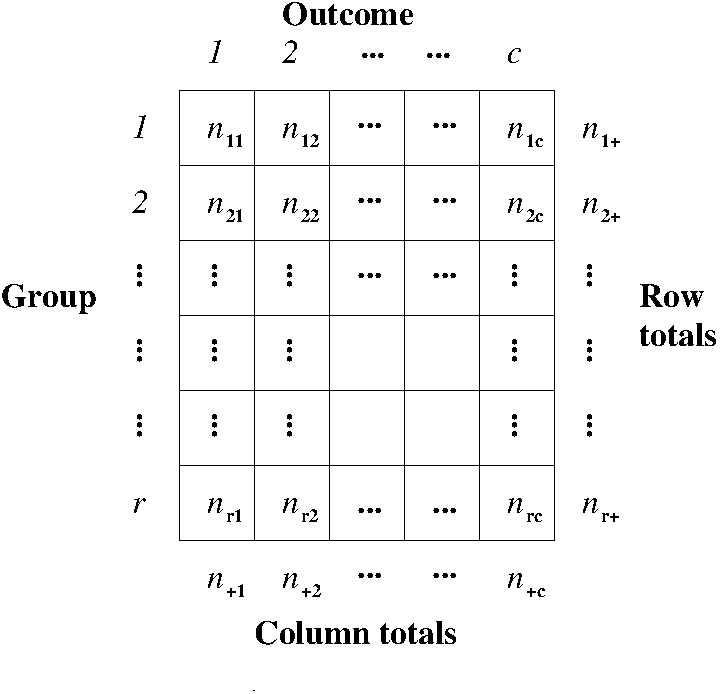
\includegraphics[scale=0.45]{Figures/table.pdf}
\end{center}

\vspace{-5mm}

$n_{ij}$ = number of subjects in group (row) $i$ and having outcome (column) $j$.\\
$n$ = $\sum\limits_{i=1}^r\sum\limits_{j=1}^c n_{ij}$ = total number of subjects.
\end{frame}


\begin{frame}
\frametitle{Tests of association in a 2-way table: $\chi^2$ test}
\framesubtitle{Deriving the $\chi^2$ test using the Poisson assumption}

The Chi\footnote{Pronounced /kai/ - a long i sound like ride}-squared $(\chi^2)$ test of independence (between row and column factors) compares the observed counts to those one would expect if there was no association between the row and column factors.

\medskip

If the row and columns factors are independent then the probability of a subject being placed in cell $(i,j)$ of the table equals the product of the probability that they are in row $i$ (i.e., level $i$ of the row factor occurs) times the probability that they are in column $j$ (i.e., level $j$ of the row factor occurs).

\medskip

You have seen the $\chi^2$ test before (I hope). Here, we are going to derive the $\chi^2$ test using what we know about the properties
of the Poisson distribution.

\end{frame}


\begin{frame}
\frametitle{Tests of association in a 2-way table: $\chi^2$ test}
\framesubtitle{Deriving the $\chi^2$ test using the Poisson assumption\ldots}
\begin{itemize}
\item Our estimate of the row $i$ probability is $\frac{n_{i+}}{n}$.
\item Our estimate of the column $j$ probability is $\frac{n_{+j}}{n}$.
\item Under the null hypothesis of row and column independence, our estimate of the cell $(i,j)$ probability is
\[ \frac{n_{i+}}{n} \times \frac{n_{+j}}{n} \]
\item So, under the null hypothesis, the expected value of the the number of subjects in cell $(i,j)$ is estimated to be
\[ \hat{n}_{ij} = n \times \frac{n_{i+}}{n} \times \frac{n_{+j}}{n} \]
\end{itemize}
\end{frame}


\begin{frame}
\frametitle{Tests of association in a 2-way table: $\chi^2$ test\ldots}
\framesubtitle{Deriving the $\chi^2$ test using the Poisson assumption\ldots}

Next we have to determine whether the residuals, $n_{ij}-\hat{n}_{ij}$, are of sufficient magnitude to provide evidence against the null hypothesis.

We do this by calculating a $Z$-statistic for each cell: \[ Z_{ij} = \frac{n_{ij}-\hat{n}_{ij}}{sd(n_{ij})} \] where $sd(n_{ij})$ is the standard deviation of $n_{ij}$.

\medskip

Now, we will utilize the assumption that the counts are Poisson distributed. Recall that Poisson count data have variance equal to the mean. We've estimated the mean to be $\hat{n}_{ij}$, so we estimate $sd(n_{ij})$ to be
\[ sd(n_{ij}) = \sqrt{\Var(n_{ij})} = \sqrt{\E(n_{ij})} \approx \sqrt{\hat{n}_{ij}} \]
and so our $Z$-statistic for cell $[i,j]$ of the table is
\[ Z_{ij} = \frac{n_{ij}-\hat{n}_{ij}}{\sqrt{\hat{n}_{ij}}} \]

\end{frame}


\begin{frame}
\frametitle{Tests of association in a 2-way table: $\chi^2$ test\ldots}
\framesubtitle{Deriving the $\chi^2$ test using the Poisson assumption\ldots}

The chi-squared test statistic is given by summing the square of the $Z_{ij}$ statistics over all cells in the table. That is,

\[X = \sum_i\sum_j\frac{ (n_{ij}-\hat{n}_{ij})^2}{ \hat{n}_{ij}} \]

Under $H_0$ (no association between rows and columns), $X$ has an approximate $\chi_{(r-1)(c-1)}^2$ distribution, where $(r-1)(c-1)$ is the degrees of freedom\footnote{Degrees of freedom are calculated as the number of independent data points minus the number of estimated parameters---can you do the maths here?}. So, for a 2-by-2 table, it is approximately $\chi_1^2$ distributed.

\end{frame}

 
\begin{frame}[fragile]
\frametitle{Tests of association in a 2-way table: $\chi^2$ test\ldots}
\framesubtitle{The $\chi^2$ test p-value}

Large values of $X$ provide evidence against $H_0$. The \pval{} is the ``probability to the right of $X$'', where the probability is from a $\chi_{(r-1)(c-1)}^2$ distribution.

\bigskip

In \rcode{R}, the probability that a $\chi_q^2$ is {\em less than} $X$ is given by \rcode{pchisq(X,q)}. The \pval{} is given by 1 minus this amount. That is,

\begin{center} \pval{} = \rcode{1-pchisq(X,q)} \end{center}

\bigskip

For a 2-by-2 table, we are working with $\chi_1^2$, so the \pval{} is the probability that a value from a $\chi_1^2$ distribution exceeds $X$. So, for a 2-by-2 table with $X=3.1$, the \pval{} would be

\begin{knitrout}\scriptsize
\definecolor{shadecolor}{rgb}{0.969, 0.969, 0.969}\color{fgcolor}\begin{kframe}
\begin{alltt}
\hlstd{> }\hlnum{1}\hlopt{-}\hlkwd{pchisq}\hlstd{(}\hlnum{3.1}\hlstd{,}\hlnum{1}\hlstd{)}
\end{alltt}
\begin{verbatim}
[1] 0.07829
\end{verbatim}
\end{kframe}
\end{knitrout}

\end{frame}

% \begin{frame}
% 
% %Plot of chi_1^2 density. Not used - doesn't look very intuitive due to long tail
% \vspace{-20mm}
% 
% x=seq(0,7,0.001)
% plot(x,dchisq(x,1),type="l",ylim=c(0,4),xaxs="i",yaxs="i")
%
% \end{frame}


\begin{frame}
\frametitle{Tests of association in a 2-way table: $\chi^2$ test\ldots}
\framesubtitle{Validity of the $\chi^2$ test}

{\bf NOTE:} The $\chi^2$ test uses the square of $Z$-statistics. These require that $n_{ij}$ is at least approximately normally distributed.

\bigskip

Recall - this requires the expected counts to be sufficiently large.

\bigskip

That is why implementations of the $\chi^2$ test often give warnings if some of the estimated expected counts ($\hat{n}_{ij}$) are ``too small''. `Too small'' is commonly taken to be $<5$.

\bigskip

If this assumption is violated then there is a solution that uses a permutation technique called  Fisher's exact test.

\end{frame}


\begin{frame}[fragile]
\frametitle{Example---Attendance/Pass}
\begin{knitrout}\scriptsize
\definecolor{shadecolor}{rgb}{0.969, 0.969, 0.969}\color{fgcolor}\begin{kframe}
\begin{alltt}
\hlstd{> }\hlkwd{chisq.test}\hlstd{(AP.tbl)}
\end{alltt}
\begin{verbatim}

	Pearson's Chi-squared test with Yates' continuity correction

data:  AP.tbl
X-squared = 24, df = 1, p-value = 9e-07
\end{verbatim}
\end{kframe}
\end{knitrout}
\medskip
This is a modified form of the chi-squared test that does a continuity correction
to the $Z_{ij}$ values, so as to correct for the fact that the cell counts
are integer valued.

\end{frame}


\begin{frame}[fragile]
\frametitle{Attendance/Pass}
\framesubtitle{Chi-squared goodness of fit test}
The standard chi-squared test (with $X$ defined as above) is given by
\begin{knitrout}\scriptsize
\definecolor{shadecolor}{rgb}{0.969, 0.969, 0.969}\color{fgcolor}\begin{kframe}
\begin{alltt}
\hlstd{> }\hlkwd{chisq.test}\hlstd{(AP.tbl,}\hlkwc{correct}\hlstd{=}\hlnum{FALSE}\hlstd{)}
\end{alltt}
\begin{verbatim}

	Pearson's Chi-squared test

data:  AP.tbl
X-squared = 26, df = 1, p-value = 3e-07
\end{verbatim}
\end{kframe}
\end{knitrout}

\medskip

In this case, both forms of the test tell us that there is massive evidence against
the null hypothesis of no association between attendance and course success.

\medskip

If the difference between the corrected and standard chi-squared tests makes any meaningful difference then you are probably up to no good!
\end{frame}


\begin{frame}[fragile]
\frametitle{Attendance/Pass\ldots}

The expected values can be obtained by saving the result of \rcode{chisq.test} as an \rcode{R} object,
and printing the \rcode{\$expected} component of it.

\begin{knitrout}\scriptsize
\definecolor{shadecolor}{rgb}{0.969, 0.969, 0.969}\color{fgcolor}\begin{kframe}
\begin{alltt}
\hlstd{> }\hlstd{AP.chisq} \hlkwb{=} \hlkwd{chisq.test}\hlstd{(AP.tbl,} \hlkwc{correct}\hlstd{=}\hlnum{FALSE}\hlstd{)}
\hlstd{> }\hlstd{AP.chisq}\hlopt{$}\hlstd{expected}
\end{alltt}
\begin{verbatim}
            Pass
Attend        fail  pass
  attend     30.14 69.86
  not.attend 13.86 32.14
\end{verbatim}
\end{kframe}
\end{knitrout}

\medskip

The actual counts for comparison:

\begin{knitrout}\scriptsize
\definecolor{shadecolor}{rgb}{0.969, 0.969, 0.969}\color{fgcolor}\begin{kframe}
\begin{alltt}
\hlstd{> }\hlstd{AP.tbl}
\end{alltt}
\begin{verbatim}
            Pass
Attend       fail pass
  attend       17   83
  not.attend   27   19
\end{verbatim}
\end{kframe}
\end{knitrout}

\end{frame}


\end{document}
